\documentclass[12pt,a4paper]{article}
\usepackage[utf8]{inputenc}
\usepackage[russian]{babel}
\usepackage[OT1]{fontenc}
\usepackage{graphicx}
\usepackage{calc}
\usepackage[margin=15mm]{geometry}
\usepackage{cmap}

% условие без картинки
\newcommand{\task}[2]{
\hrule
\hbox to \textwidth {%
     \vrule
\parbox[t]{0.04\textwidth}{\smallskip \centering #1}%
     \vrule%
\hfill%
     \parbox[t]{0.93\textwidth}{\smallskip #2 \smallskip}\hfill%
\vrule
}
\hrule
    \pagebreak[2]
}

\newlength{\h}
\newsavebox{\taskbox}
\newlength{\x}
\newsavebox{\pictbox}

% условие с картинкой (картинка выравнивается по центру)
\newcommand{\taskpic}[3]{
\savebox{\taskbox}{\parbox[t]{0.93\textwidth-4.3cm}{\smallskip #2 \smallskip}}
\savebox{\pictbox}{\parbox[t]{4cm}{\smallskip \centering
     \vspace{0pt} #3 \smallskip}}
\h=\ht\taskbox
\advance\h\dp\taskbox
\x=\ht\pictbox
\advance\x\dp\pictbox
\hrule
\hbox to \textwidth {%
\vrule\parbox[t][\maxof{\h}{\x}][t]{0.04\textwidth}{ \smallskip
     \centering #1 }\vrule%
\hfill\parbox[t][\maxof{\h}{\x}][t]{0.93\textwidth-4.3cm}{\smallskip #2
     \smallskip}\hfill\vrule%
\hfill\parbox[t][\maxof{\h}{\x}][c]{4cm}{\hfil #3 \hfil}\hfill\vrule
}
\hrule
\pagebreak[2]
}
\pagestyle{empty}
\graphicspath{ {images/} }

\begin{document}

\begin{center}
\begin{Large}
\textsc{ГЦФО. 9 класс. 2014/15.}
\end{Large}
\end{center}

\small

\taskpic[6cm]{18}{На примусе, расходующем $\mu = 0{,}1$~кг бензина в час, стоит котелок, в котором находится $m = 1$~кг воды. График зависимости тепловой мощности $P$, выделяемой в окружающую среду, от времени приведен на рисунке. Постройте график зависимости температуры воды в котелке от времени. Теплоемкость котелка $C = 800$~Дж/$^\circ$C, удельная теплоемкость воды $c_0 = 4200$~Дж/(кг$\cdot^\circ$C). Удельная теплота сгорания бензина $q = 43$~МДж/кг. Начальная температура воды $T=20^\circ$C. Принять, что в любой момент времени температура котелка и воды совпадают.}{
\begin{tikzpicture}
\begin{axis}[
    width=6cm,
    xmax=10.5,
    ymax=1000,
    xtick={0,2,...,10},
    ytick={0,200,...,1000},
    grid=both,
    minor tick num=3,
    major grid style=thick,
    minor grid style=thin,
    axis lines=middle,
    axis line style={->},
    xlabel={$t$, мин},
    ylabel={$P$, Вт},
    /pgf/number format/1000 sep={\,},
]
\addplot[thick,domain=0:10] {1200 * (1 - exp(-x/7))};
\end{axis}
\end{tikzpicture}
}
\task{22}{Утюг устроен следующим образом: его нагреватель выключается, если температура утюга становится больше некоторой температуры $t_2$, и включается, как только его температура падает ниже $t_1$ (эти температуры неизвестны). Если включенный утюг стоит с открытой металлической поверхностью, его нагреватель работает в среднем $k=1/4$ всего времени. При этом мощность теплоотдачи можно считать постоянной. Если утюгом начинают гладить, то промежуток времени между последовательными моментами включения нагревателя становится в $n=4/3$ раза меньше. В этом случае мощность теплоотдачи также остается постоянной. Какую часть времени он работает в среднем во втором случае?}
\taskpic{23}{Школьница Василиса проводит опыты с пружиной. Сначала Василиса обнаружила, что длина пружины в нерастянутом состоянии составляет 10 см, а груз массой $m$~г, подвешенный к пружине, дополнительно растягивает ее на $0{,}01m$~см. Затем Василиса подвесила пружину с грузом над сосудом в форме прямоугольного параллелепипеда, как показано на рисунке, и стала наливать в сосуд воду. Груз имеет форму куба длиной ребра 10~см, его плотность равна плотности воды. В начале опыта расстояние от нижней грани груза до дна сосуда составляет 30~см. Площадь основания сосуда составляет 1000~см$^2$. Нижняя грань куба во время опыта сохраняла горизонтальное положение. Постройте график зависимости длины пружины $l$ от объема воды $V$, налитой в сосуд. При каких значениях объема $V$ груз находился в воздухе? был частично погружен в воду? был полностью погружен в воду?}{
\begin{tikzpicture}[scale=0.5]
\draw[interface] (1,8)--(3,8);
\draw (2,8) -- (2,7);
\draw[spring] (2,7) -- (2,5);
\draw (2,5) -- (2,4);
\draw (1.5,4) rectangle (2.5,3);
\draw (0,6) -- (0,0) -- (4,0) -- (4,6);
\end{tikzpicture}
}
\task{24}{Фонтан в Женеве бьет на высоту $h$. Расход воды составляет $P$ кг за 1 секунду. Найдите площадь сечения сопла фонтана. Ускорение свободного падения равно $g$, плотность жидкости $\rho$. Пренебречь сопротивлением воздуха, поверхностным натяжением и вязкостью жидкости.}
\taskpic{25}{На горизонтальный скользкий цилиндр аккуратно, без зазоров намотали широкую ленту. На оба конца ленты подвесили одинаковые грузики массы $m$. Давление ленты на цилиндр при этом оказалось равно $P$. Найдите диаметр окружности цилиндра. Ширина ленты $l$, ускорение свободного падения $g$. Массой ленты по сравнению с массой грузов пренебречь, трение ленты о саму себя и о цилиндр отсутствует. Ширина ленты много меньше диаметра окружности цилиндра.}{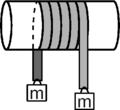
\includegraphics[width=3cm]{25}}
\taskpic{26}{Шар массы $m_1$ налетает со скоростью $v$ на покоящийся шар массы $m_2$. Между ними происходит центральный, абсолютно упругий удар. Какая часть кинетической энергии первого шара перейдет ко второму? Постройте график зависимости доли переданной энергии от массы $m_2$.}{
\begin{tikzpicture}
\draw (0,0) circle [radius=0.3] node[below=0.3cm,anchor=north] {$m_1$};
\draw[->] (0.3,0) -- (1.3,0) node[midway,anchor=north] {$\vec{v}$};
\draw (2.5,0) circle [radius=0.5] node[below=0.5cm,anchor=north] {$m_2$};
\end{tikzpicture}
}
\end{document}
